
%Copyright 2014 Jean-Philippe Eisenbarth
%This program is free software: you can 
%redistribute it and/or modify it under the terms of the GNU General Public 
%License as published by the Free Software Foundation, either version 3 of the 
%License, or (at your option) any later version.
%This program is distributed in the hope that it will be useful,but WITHOUT ANY 
%WARRANTY; without even the implied warranty of MERCHANTABILITY or FITNESS FOR A 
%PARTICULAR PURPOSE. See the GNU General Public License for more details.
%You should have received a copy of the GNU General Public License along with 
%this program.  If not, see <http://www.gnu.org/licenses/>.

%Based on the code of Yiannis Lazarides
%http://tex.stackexchange.com/questions/42602/software-requirements-specification-with-latex
%http://tex.stackexchange.com/users/963/yiannis-lazarides
%Also based on the template of Karl E. Wiegers
%http://www.se.rit.edu/~emad/teaching/slides/srs_template_sep14.pdf
%http://karlwiegers.com
\documentclass{scrreprt}
\usepackage{listings}
\usepackage{underscore}
\usepackage{float}
\usepackage{graphicx}
\usepackage{epstopdf}
\usepackage{booktabs}
\usepackage{xcolor}
\usepackage[bookmarks=true]{hyperref}
\usepackage[utf8]{inputenc}
\usepackage[english]{babel}
\hypersetup{
    bookmarks=true,    % show bookmarks bar?
    pdftitle={Software Requirement Specification for Recipe Buddy},    % title
    pdfauthor={Matthew Sprague, Brian Williams, Joseph Morrison, Jeffrey Rescignano},                     % author
    pdfsubject={Software Requirement Specification},                        % subject of the document
    pdfkeywords={Recipe, Buddy, Software, Requirement, Specification}, % list of keywords
    colorlinks=true,       % false: boxed links; true: colored links
    linkcolor=black,       % color of internal links
    citecolor=black,       % color of links to bibliography
    filecolor=black,        % color of file links
    urlcolor=black,        % color of external links
    linktoc=page            % only page is linked
}%
\def\myversion{1.6}
%\title
\usepackage{hyperref}
\usepackage{glossaries}

\makeglossaries

% Define Recipe Buddy itself
\newglossaryentry{Recipe Buddy}
{
	name={Recipe Buddy},
	description={Is the software defined by this document}
}

% Software related to the document
\newglossaryentry{LaTeX}
{
    name=LaTeX,
    description={Is the markup language used to prepare the document}
}

% Software used by Recipe Buddy
\newglossaryentry{Python}
{
	name=Python,
	description={Is a scripting langugage used by \gls{Recipe Buddy}}
}

\newglossaryentry{Flask}
{
	name=Flask,
	description={Is a \gls{Python}-based web framework used by \gls{Recipe Buddy}}
}

\newglossaryentry{MariaDB}
{
	name=MariaDB,
	description={Is a database framework used by \gls{Recipe Buddy}}
}

\newglossaryentry{SQL}
{
	name=SQL,
	description={Is the language used by \gls{MariaDB} to communicate with a database}
}

\newglossaryentry{Docker}
{
	name=Docker,
	description={Is software providing a virtual platform, or ``container," on which \gls{Recipe Buddy} resides}
}

\newglossaryentry{Docker Compose}
{
	name={Docker Compose},
	description={Is a tool used to manage multiple \gls{Docker} containers and run them as a single application}
}

\newglossaryentry{HTML}
{
	name=HTML,
	description={Is a language used to describe the structure of a webpage}
}

\newglossaryentry{JavaScript}
{
	name=JavaScript,
	description={Is a language used to describe the functions of a webpage}
}

\newglossaryentry{CSS}
{
	name=CSS,
	description={Is a language used to describe the appearance of a webpage}
}

\newglossaryentry{Bootstrap}
{
	name=Bootstrap,
	description={Is a \gls{frontend} web development toolkit used by \gls{Recipe Buddy}}
}

% Definitions related to cybersecurity
\newglossaryentry{SQL injection}
{
	name={SQL injection},
	description={Refers to the process of hacking a database where a user runs their own malicious \gls{SQL} code. \emph{see} \gls{SQL}}
}

\newglossaryentry{XSS injection}
{
	name={XSS injection},
	description={Refers to the process of hacking a website where a user inserts their own malicious code into a website.
	This malicious code can then be run by users of that same website}
}

% Definitions related to documentation
\newglossaryentry{pdoc}
{
	name=pdoc,
	description={Is a \gls{Python} library used to generate \gls{documentation} of \gls{Python} code.}
}

\newglossaryentry{documentation}
{
	name=documentation,
	description={Refers to software's technical documents}
}

% Other "software" definitions --- maybe this isn't
% software, per se, but it is related. Things like
% protocols, algorithms, and APIs go here.
\newglossaryentry{ECMAScript}
{
	name=ECMAScript,
	description={Is a set of rules and constraints that define \gls{JavaScript}}
}

\newglossaryentry{HTTPs}
{
	name=HTTPs,
	description={Is a protocol providing secure communication to a website}
}

\newglossaryentry{RESTful API}
{
	name={RESTful API},
	description={Is a set of specifications and constraints for web communication}
}

\newglossaryentry{serialization}
{
	name=serialization,
	description={Is the process of converting a program's internal data into storable and transmittable data}
}

\newglossaryentry{serialized}
{
	name=serialized,
	description={\emph{See} \gls{serialization}}
}

\newglossaryentry{frontend}
{
	name=frontend,
	description={Is the layer of software presented to an end user}
}

\newglossaryentry{backend}
{
	name=backend,
	description={Is the layer of software that manages \gls{Recipe Buddy}'s internal functions. It is hidden from an end user}
}

\newglossaryentry{unit testing}
{
	name={unit testing},
	description={Is a method of software testing where every function is tested individually}
}

\newglossaryentry{Functional Requirements}
{
	name={Functional Requirements},
	description={describe the services that \gls{Recipe Buddy} must offer}
}

\newglossaryentry{Nonfunctional Requirements}
{
	name={Nonfunctional Requirements},
	description={describe the systems that \gls{Recipe Buddy} must be built on}
}


% Legal definitions
\newglossaryentry{COPPA}
{
	name=COPPA,
	description={Is a federal law in the U.S. that governs how to operate a website accessed by children under the age of thirteen}
}

\newglossaryentry{CCPA}
{
	name=CCPA,
	description={Is a state law in California that governs how websites handle user data}
}


\begin{document}

\begin{flushright}
    \rule{16cm}{5pt}\vskip1cm
    \begin{bfseries}
        \Huge{SOFTWARE REQUIREMENTS\\ SPECIFICATION}\\
        \vspace{1.85cm}
        for\\
        \vspace{1.85cm}
        $Recipe Buddy$\\
        \vspace{1.8cm}
        \LARGE{Version \myversion}\\
        \vspace{1.8cm}
        Prepared by $ $Matthew Sprague, Brian Williams, Joseph Morrison, Jeffrey Rescignano$ $\\
        \vspace{1.8cm}
        $ $Certified Data Boys$ $\\
        \vspace{1.8cm}
        \today\\
    \end{bfseries}
\end{flushright}

\tableofcontents

\chapter*{Revision History}\label{revisions}

\begin{center}
    \begin{tabular}{c c c c}
        \midrule
        Name             & Date       & Reason For Changes & Version \\
        \midrule
        All team members & Oct 8 2021 & Initial doc        & 1.0     \\
        \midrule
        Matthew Sprague
                         & Oct 20 2021
                         & Updated dependencies \& glossary
                         & 1.1                                       \\
        Matthew Sprague
                         & Oct 28 2021
                         & Updated dependencies
                         & 1.2                                       \\
        \midrule
        
        Brian Williams
                         & November 5 2021
                         & Update requirement specification
                         & 1.3                                       \\
        
        Brian Williams
                         & November 17 2021
                         & Update requirement specification
                         & 1.4                                       \\
        
        Brian Williams
                         & December 5 2021
                         & Update Update stimulus and response
                         & 1.5                                       \\
        
        Brian Williams
                         & December 12 2021
                         & Update requirement description
                         & 1.6                                       \\
        \midrule
    \end{tabular}
\end{center}

\chapter{Introduction}

\section{Purpose}
$ $\gls{Recipe Buddy} is a modern recipe sharing website intended to facilitate connections between our users with food and culinary arts.
It creates a personalized experience for the user, showcases popular and trending recipes, and creates a community through various recipe sharing services.$ $

\section{Document Conventions}
$ $The SRS document has the following conventions:$ $
\subsection{Lists}
$ $Lists and sublists should be formatted as such:
\begin{itemize}
    \item This is an entry on a list!
    \item This is another entry on a list.
          \begin{itemize}
              \item This is an entry on a nested list!
              \item This is another entry on a nested list.
                    \begin{itemize}
                        \item And this is an item on a doubly nested list.
                    \end{itemize}
          \end{itemize}
\end{itemize}
Lists should never be nested more than twice.
The list in this section shows how far we allow our lists to go.
Anything more than that is not allowed.

\subsection{Revisions}
After a new revision, it is important to log your progress.
Please update this document's version number and update this document's Revision History table.

\subsection{Styling}
When updating this document, adhere to the following style guidelines:
\begin{itemize}
    \item The first paragraph of each section or subsection does not need to be indented.
          Subsequent paragraphs should be indented.
          In \gls{LaTeX}, that is done by default by typing two blank spaces ``\ \ " after a paragraph.
    \item This document should be typed using the default \gls{LaTeX} font and styling.
    \item When writing numbers within a paragraph:
          \begin{itemize}
              \item Whole numbers between zero and fifteen should be typed alphaetically.
              \item Whole numbers equal to or above 16 should be typed numerically.
              \item Decimal numbers, such as 3.14, should be typed numerically.
              \item Fractions should be typed in the form {$\frac{1}{2}$}.
                    In \gls{LaTeX}, this can be done using the following code:
                    \\ \texttt{ \{\$ \textbackslash frac\{1\}\{2\} \$\} }
          \end{itemize}
\end{itemize}

\subsection{Code}
When writing code within a paragraph:
\begin{itemize}
\item For short snippets, it is okay to use inline code. For example: \\
The \gls{Python} command \texttt{ print( ... ) } writes to standard output. \\
In \gls{LaTeX}, this is done using the \texttt{ \textbackslash texttt\{ \} } command in-line with the rest of a paragraph.
\item For longer snippets, please give the code its own block. For example: \\
The following \gls{Python} function will calculate the area of a circle: \\
\begin {verbatim}
import math

// This function takes in the radius of a circle
// and returns the area of that circle.
def area_circle(radius):

r_squared = radius ** 2
return math.pi * r_squared
\end{verbatim}
This can be done by using a \texttt{ verbatim } block in \gls{LaTeX}.  

Please remember that this is a requirements document, and not the system's \gls{documentation}!
Remember to only use code in this document when it is needed!
That is,
\begin{itemize}
    \item Write code that clearly illustrates what you are doing.
    \item Write code that is concise.
    \item Explain what your code is doing such that a reader with minimal technical skill can understand what the code is doing.
    \item If the code takes too long to explain, save it for the system's \gls{documentation}.
    \item Try not to take up more than half of a page with a block of code.
    \item Never take up more than an entire page with a block of code.
    \item Aim to have minimal overlap between the code in this document and the code in our system's \gls{documentation}.
    \item The code in this document must convey meaningful information to all readers.
          It should be useful for developers, as well as non-developers.
\end{itemize}
\end{itemize}
$ $

\section{Intended Audience and Reading Suggestions}
$ $This document is aimed at a wide audience:
\begin{itemize}
    \item \gls{Recipe Buddy} developers should be able to go over this document to understand how the system functions.
          Developers should have the ability to use this in conjunction with the system's \gls{documentation} to gain a comprehensive understanding of the system's underlying features and overall design.
          Developers should also be able to use this document to understand who to design this system for and why the system is designed the way it is.
          That way, with each new proposed update to \gls{Recipe Buddy}, developers can assess if it would align with the system's design philosphy.
    \item \gls{Recipe Buddy} designers and clients should be able to go over this document to understand how the system is designed.
          With any proposed updates or revisions to the system, designers should have the ability to refer to this document and ensure such changes align with \gls{Recipe Buddy}'s design philosophy.
\end{itemize}
$ $

\section{Project Scope}
\gls{Recipe Buddy} is a tool that allows registered users to organize their own recipies, view recipies of other registered users, and keep a catalog of food, kitchenware and applicances that they own. \gls{Recipe Buddy} can also track dietary restrictions to offer a better user experince.
$ $\gls{Recipe Buddy} organizes recipies by:
\begin{itemize}
    \item Allowing users to create a recipe.
    \item Allowing users to modify their recipies.
    \item Allowing users to delete their recipies.
    \item Allowing users to set the visibility of their recipies (i.e.\ public or private)
    \item Allowing users to share private recipies with specific users.
    \item Allowing users to offer suggestions to other's recipies.
\end{itemize}
$ $
$ $\gls{Recipe Buddy} keeps a catalog of food and kitchenware items by:
\begin{itemize}
    \item Allowing for a detailed list of food items available in a users panty.
    \item Allowing for a user to add all items from a particular recipe into their panty.
    \item Allowing for users to keep a detailed list of kitchenware that they own.
    \item Allowing users to edit or modify these lists at any time from the user menu.
\end{itemize}
$ $
$ $\gls{Recipe Buddy} tracks dietary restrictions by:
\begin{itemize}
    \item Allowing users to keep a detailed list of specific ingredients marked as allergens.
    \item Allowing users to keep a detailed list of restricted categories. (i.e.\ dairy for lactose intolerant or bread for gluten-free).
\end{itemize}
$ $

\section{References}
Throughout this document, mutliple web addresses are referred to in order to give a better description of the \gls{Recipe Buddy} software.

\begin{itemize}
    \item Reference 1
          \begin{itemize}
              \item Name: Chrome Browser System Requirements
              \item Author: Google
              \item Version: 95.0.4638.32
              \item Access Date: September 29, 2021
              \item Location: \href{https://support.google.com/chrome/a/answer/7100626?hl=en}{support.google.com}
          \end{itemize}
    \item Reference 2
          \begin{itemize}
              \item Name: Firefox Browser System Requirements
              \item Author: Mozilla
              \item Version: 92.0
              \item Access Date: October 4, 2021
              \item Location: \href{https://www.mozilla.org/en-US/firefox/92.0.1/system-requirements/}{www.mozilla.org}
          \end{itemize}
\end{itemize}

\chapter{Overall Description}

\section{Product Perspective}
\gls{Recipe Buddy} is a multi-functional tool for organizing recipes, pantry items and dietary restrictions.
Although several recipe websites already exist, \gls{Recipe Buddy} offers many powerful customizations and search features that seperate it from the competition.

\section{Product Functions}
$ $The \gls{Recipe Buddy} software offers:
\begin{itemize}
    \item A limited publicly-accessible database of Recipes.
    \item User registration to access full features of the website.
    \item The organization of recipies by:
          \begin{itemize}
              \item Allowing users to create a recipe.
              \item Allowing users to modify their recipies.
              \item Allowing users to delete their recipies.
              \item Allowing users to set the visibility of their recipies (i.e.\ public or private)
              \item Allowing users to share private recipies with specific users.
              \item Allowing users to offer suggestions to other's recipies.
          \end{itemize}
    \item The organization of panty items and cookware by:
          \begin{itemize}
              \item Allowing for a detailed list of food items available in a users panty.
              \item Allowing for a user to add all items from a particular recipe into their panty.
              \item Allowing for users to keep a detailed list of kitchenware that they own.
              \item Allowing users to edit or modify these lists at any time from the user menu.
          \end{itemize}
    \item The tracking of dietary restrictions by:
          \begin{itemize}
              \item Allowing users to keep a detailed list of specific ingredients marked as allergens.
              \item Allowing users to keep a detailed list of restricted categories. (i.e.\ dairy for lactose intolerant or bread for gluten-free).
          \end{itemize}
    \item Powerful search features to sort and filter:
          \begin{itemize}
              \item By pantry and cookware items already available to the user.
              \item By user-specified dietary restrictions.
              \item By popularity, rating or difficulty.
          \end{itemize}
    \item Social features such as:
          \begin{itemize}
              \item Private sharing of a recipe.
          \end{itemize}
\end{itemize}
$ $

\section{User Classes and Characteristics}
Guest:
\begin{itemize}
    \item A guest is defined as someone browsing the \gls{Recipe Buddy} website, but have not created a user account or signed in.
    \item Guests have limited access to the resources available on \gls{Recipe Buddy}.
          \begin{itemize}
              \item Guests will not be able to access various parts of the software tutorial videos.
              \item Guests are not allowed to cook recipes.
              \item Guests are not allowed to store user-specific data such as dietary restrictions, favorited recipes, pantry items or cookware items.
              \item Guests cannot leave comments or reviews on recipies.
              \item Guests cannot upload or contribute recipes to the \gls{Recipe Buddy} database.
              \item Guests cannot access powerful search features.
              \item Guests cannot view private recipes shared with them.
          \end{itemize}
\end{itemize}

User:
\begin{itemize}
    \item A user is defined as someone browsing or contributing to the \gls{Recipe Buddy} website, who has registed a user account ans signed in.
    \item Users have full access to the resources available on \gls{Recipe Buddy}.
          \begin{itemize}
              \item Users can view the full video tutorial on how to access \gls{Recipe Buddy} features.
              \item Users can cook recipes.
              \item Users can store user-specific data such as dietary restrictions, favorited recipes, pantry items or cookware items.
              \item Users can leave comments and reviews on recipies.
              \item Users can upload and contribute recipes to the \gls{Recipe Buddy} database.
              \item Users can access powerful search features.
              \item Users can access private recipies shared with them.
          \end{itemize}
\end{itemize}

\section{Operating Environment}
Although \gls{Recipe Buddy} is expected to work on modern browsers, the \gls{Recipe Buddy} client will only be tested extensively to ensure proper functionality across the top three major web browsers by marketshare including:
\begin{itemize}
    \item Google Chrome (Desktop)
    \item Apple Safari (Desktop)
    \item Mozilla Firefox (Desktop)
\end{itemize}

\section{Design and Implementation Constraints}
\gls{Recipe Buddy} shall abide by the following legal constraints:
\begin{itemize}
    \item Children's Online Privacy Protection Act (\gls{COPPA})
    \begin{itemize}
        \item \gls{Recipe Buddy} shall not allow children, as defined by \gls{COPPA}, to register for the service.
        \item \gls{COPPA} defines a child as anyone under the age of 13.
    \end{itemize}
    \item California Consumer Privacy Act (\gls{CCPA})
    \begin{itemize}
        \item \gls{Recipe Buddy} will allow users to query their personal information, as collected by \gls{Recipe Buddy}.
        \item \gls{Recipe Buddy} will allow users to delete their account and all of the information attached to it.
        \item \gls{Recipe Buddy} cannot sell a user's information.
        \item \gls{Recipe Buddy} cannot treat a user exercising their \gls{CCPA} rights any different from other users.
    \end{itemize}
\end{itemize}  

\gls{Recipe Buddy} shall also abide by the following technical constraints:
\begin{itemize}
    \item \gls{Recipe Buddy} shall be written with the following programming languages and frameworks:
    \begin{itemize}

        \item \gls{Python}
        \begin{itemize}

            \item Version 3.9.7 or newer
            \item Webpage: \href{https://www.python.org/}{www.python.org}
            \item \Gls{documentation}: \href{https://docs.python.org/3.9/}{docs.python.org}
            \item Download: \href{https://www.python.org/downloads/release/python-397/}{www.python.org}

        \end{itemize}

        \item \gls{MariaDB}
        \begin{itemize}

            \item Version 10.6.4 or newer
            \item Webpage: \href{https://mariadb.org/}{mariadb.org}
            \item \Gls{documentation}: \href{https://mariadb.com/kb/en/}{mariadb.org}
            \item Download: \href{https://mariadb.org/download/?tab=mariadb&release=10.6.4&product=mariadb}{mariadb.org}
        
        \end{itemize}
        
        \item \gls{HTML}5
        \begin{itemize}
        
            \item \Gls{documentation}: \href{https://developer.mozilla.org/en-US/docs/Web/HTML}{developer.mozilla.org}
        
        \end{itemize}
        
        \item \gls{CSS}3
        \begin{itemize}
        
            \item \Gls{documentation}: \href{https://developer.mozilla.org/en-US/docs/Web/CSS}{developer.mozilla.org}
        
        \end{itemize}

        \item \gls{JavaScript}
        \begin{itemize}

            \item Specified by \gls{ECMAScript} 2021
            \item \gls{JavaScript} \gls{documentation}: \href{https://developer.mozilla.org/en-US/docs/Web/JavaScript}{developer.mozilla.org}
            \item \gls{ECMAScript} 2021 \gls{documentation}: \href{https://www.ecma-international.org/wp-content/uploads/ECMA-262_12th_edition_june_2021.pdf}{www.ecma-international.org}

        \end{itemize}
        
        \item \gls{Docker}
        \begin{itemize}
        
            \item Version 20.10.9 or newer
            \item Website: \href{https://www.docker.com/}{docker.com}
            \item \Gls{documentation}: \href{https://docs.docker.com/get-started/overview/}{docs.docker.com}
            \item Source code: \href{https://github.com/moby/moby}{github.com}
            \item Download: \href{https://docs.docker.com/get-docker/}{docs.docker.com}
        
        \end{itemize}
        
        \item \gls{Docker Compose}
        \begin{itemize}
        
            \item Version 2.0.1 or newer
            \item \Gls{documentation}: \href{https://docs.docker.com/compose/}{docs.docker.com}
            \item Source code: \href{https://github.com/docker/compose}{github.com}
            \item Download: \href{https://docs.docker.com/compose/install/}{docs.docker.com}
        
        \end{itemize}

        \item \gls{MariaDB} Connector/\gls{Python}
        \begin{itemize}

            \item Version 1.0.7 or newer
            \item \Gls{documentation}: \href{https://mariadb-corporation.github.io/mariadb-connector-python/}{mariadb-corporation.github.io}
            \item Source code: \href{https://github.com/mariadb-corporation/mariadb-connector-python}{github.com}

        \end{itemize}

        \item \gls{Flask}
        \begin{itemize}

            \item Version 2.0.2 or newer
            \item Webpage: \href{https://flask.palletsprojects.com/en/2.0.x/}{flask.palletsprojects.com}
            \item \Gls{documentation}: \href{https://flask.palletsprojects.com/en/2.0.x/api/}{flask.palletsprojects.com}
            \item Source code: \href{https://github.com/pallets/flask}{github.com}

        \end{itemize}
        
        \item \gls{Flask}-SQLAlchemy
        \begin{itemize}
        
        	\item Version 2.5.1 or newer
        	\item Webpage: \href{https://flask-sqlalchemy.palletsprojects.com/en/2.x/}{flask-sqlalchemy.palletsprojects.com}
        	\item \Gls{documentation}: \href{https://flask-sqlalchemy.palletsprojects.com/en/2.x/api/}{flask-sqlalchemy.palletsprojects.com}
        	\item Source code: \href{https://github.com/pallets/flask-sqlalchemy}{github.com}
        
        \end{itemize}
        
        \item \gls{Flask}-login
        \begin{itemize}
        
        	\item Version 0.5.0 or newer
        	\item \Gls{documentation}: \href{https://flask-login.readthedocs.io/en/latest/}{flask-login.readthedocs.io}
        	\item Source code: \href{https://github.com/maxcountryman/flask-login}{github.com}
        
        \end{itemize}
        
        \item \Gls{Flask}-WTF
        \begin{itemize}
        
        	\item Version 0.15.1 or newer
        	\item \Gls{documentation}: \href{https://flask-wtf.readthedocs.io/en/0.15.x/}{flask-wtf.readthedocs.io}
        	\item Source code: \href{https://github.com/wtforms/flask-wtf}{github.com}
        
        \end{itemize}
        
        \item python-email-validator
        \begin{itemize}
        
        	\item Version 1.1.3 or newer
        	\item Source code: \href{https://github.com/JoshData/python-email-validator}{github.com}
        
        \end{itemize}
        
        \item pdoc
        \begin{itemize}

            \item Version 8.0.0 or newer
            \item Webpage: \href{https://pdoc.dev/}{pdoc.dev}
            \item \Gls{documentation}: \href{https://pdoc.dev/docs/pdoc.html}{pdoc.dev}
            \item Source code: \href{https://github.com/mitmproxy/pdoc}{github.com} 

        \end{itemize}
        
        \item pyyaml
        \begin{itemize}
        
            \item Version 6.0 or newer
            \item Webpage: \href{https://pyyaml.org/}{pyyaml.org}
            \item \Gls{documentation}: \href{https://pyyaml.org/wiki/PyYAMLDocumentation}{pyyaml.org}
            \item Source code: \href{https://github.com/yaml/pyyaml}{github.com}
        
        \end{itemize}
        
        \item libyaml
        \begin{itemize}
        
            \item Version 0.2.5 or newer
            \item Webpage: \href{https://pyyaml.org/wiki/LibYAML}{pyyaml.org}
            \item \Gls{documentation}: \href{https://libyaml.docsforge.com/}{libyaml.docsforge.com}
            \item Source code: \href{https://github.com/yaml/libyaml}{github.com}
        
        \end{itemize}
        
        \item \gls{Bootstrap}
        \begin{itemize}

            \item Version 5.1 or newer
            \item Webpage: \href{https://getbootstrap.com/}{getbootstrap.com}
            \item \Gls{documentation}: \href{https://getbootstrap.com/docs/5.1/getting-started/introduction/}{getbootstrap.com}
            \item Source code: \href{https://github.com/twbs/bootstrap}{github.com}
            \item Download: \href{https://getbootstrap.com/docs/5.1/getting-started/download/}{getbootstrap.com}

        \end{itemize}

    \end{itemize}


    \item \gls{Recipe Buddy} will interface with its \gls{MariaDB} database using a \gls{RESTful API} and \gls{SQL} code.
    \begin{itemize}

        \item \gls{RESTful API} specifications: \href{https://restfulapi.net/}{restfulapi.net}
    
    \end{itemize}

    \item \gls{Recipe Buddy} should be designed to save recipe data very quickly.
    \begin{itemize}

        \item Recipe data should be locally cached as it is entered by the user.
        \item \gls{Recipe Buddy} will provide a button to save recipe data on the edit recipe page.
        \item When the user decides to save a recipe, recipe data should be \gls{serialized} in no more than 0.5 seconds on a modern computer.
        \item Immediately following \gls{serialization}, the recipe data should be uploaded to the database.
        \item When a recipe is saved, the user should be notified. This should occur no longer than 5 seconds after the user clicks the button to save their recipe, assuming that the user has a stable connection and is using a modern computer.

    \end{itemize}

    \item The data stored by \gls{Recipe Buddy} must abide by the following constraints:
    \begin{itemize}

        \item Uploaded images must be stored in .jpg, .png, or .webp file formats.
        \item Uploaded videos must be stored in .mp4, .mov, or .webm file formats.
        \item Uploaded files must be no more than 4MB in size.

    \end{itemize}

\end{itemize}

\section{User Documentation}
\gls{Recipe Buddy} will feature a web-based video tutorial that will help wesbite users and visitors explore \gls{Recipe Buddy} features. The \gls{Recipe Buddy} software also features a support page with multiple FAQ questions and how-to tutorials.

\section{Assumptions and Dependencies}
\gls{Recipe Buddy} is designed under the following assumptions:
\begin{itemize}
    \item Users will not try to use \gls{Recipe Buddy} on an unsupported browser.
    \item All specified languages and frameworks are fully up to date and working on \gls{Recipe Buddy}'s host server.
    \item A server hosting \gls{Recipe Buddy} must have reliable internet connectivity, and it must have enough space to store \gls{Recipe Buddy}'s database.
    \item A user signing up for \gls{Recipe Buddy} will have an email with which to create their account.
\end{itemize}

\chapter{External Interface Requirements}

\section{User Interfaces}
Buttons included on every page:
\begin{itemize}
    \item Home
    \item Search
    \item Profile
    \item New Recipe
\end{itemize}

\section{Hardware Interfaces}
The Recipe Buddy client requires a modern web browser to access.

Please refer to the web browser's minimum specifications in order to get an idea of the required hardware.

\begin{itemize}
    \item \href{https://support.google.com/chrome/a/answer/7100626?hl=en}{Google Chrome Web Browser System Requirements}
    \item Apple Safari Web Browser System Requirements
          \begin{itemize}
              \item Apple Safari is pre-installed on all Apple Computers by default. Minimum system requirements include a modern macOS computer system.
          \end{itemize}
    \item \href{https://www.mozilla.org/en-US/firefox/92.0.1/system-requirements/}{Mozilla Firefox System Requirements}
\end{itemize}

\section{Software Interfaces}
The \gls{Recipe Buddy} client software relies on a web browser in order to properly fetch and display data within the \gls{Recipe Buddy} sytem. Web browers are not operating system restricted as they run on all major operating systems.

\section{Communications Interfaces}
The \gls{Recipe Buddy} client software interface runs in a web browser and communicates via the \gls{HTTPs} protocol. An internet connection of speed 2.5Mbps - 5Mbps is required to use the full features of \gls{Recipe Buddy} such as the video tutorial and embedded videos within recipes.

\chapter{System Features}

\section{Recipe: Recipe Creation}

\subsection{Description and Priority}

The recipe creation feature allows registered users to upload recipes to the \gls{Recipe Buddy} recipe database. Various attributes about the recipe such as ingredients, instrctions, videos, images, cook time, cook temperature can be set by the user.

\begin{center}
    \begin{tabular}{| c | c | c | c |}
        \hline
        Critical Level  & High                                                                 \\
        \hline
        Dependencies    & N/A                                                                  \\
        \hline
        Estimated Time  & 1 week - 2 weeks                                                     \\
        \hline
        Lead Developers & Matthew Sprague, Jeffrey Rescignano \\
        \hline
        Testing         & Client and focus group \gls{frontend} testing,
                          \gls{unit testing} for \gls{backend}                                 \\
        \hline
        Risks           & None                                                                 \\
        \hline
    \end{tabular}
\end{center}

\subsection{Stimulus/Response Sequences}

\begin{figure}[H]\centering
    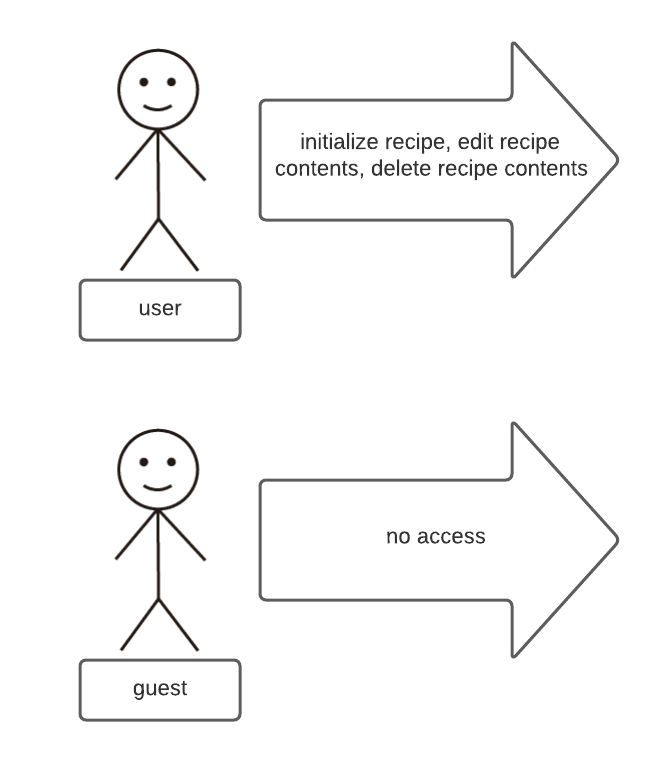
\includegraphics[width=\columnwidth]{response diagrams/Recipe Creation.png}
\end{figure}

\subsection{\gls{Functional Requirements}}

\begin{itemize}
    \item REQ-1.1.1: Edit various elements of the recipe:
          \begin{itemize}
              \item Ingredients
              \item Time
              \item Temperature
              \item Pictures
              \item Videos
              \item Instructions
          \end{itemize}
    \item REQ-1.1.2: Delete the selected recipe.
    \item REQ-1.1.3: Share the selected recipe:
          \begin{itemize}
              \item Private sharing
              \item Public sharing
          \end{itemize}
\end{itemize}

\section{Recipe: Recipe Pages}

The recipe pages feature allows both guests and registered users to view recipe information from the \gls{Recipe Buddy} recipe database. Guests can only view public recipes, while registered users can view public recipes, their own private recipes and other private recipes shared to them by other users.

\subsection{Description and Priority}
\begin{center}
    \begin{tabular}{| c | c | c | c |}
        \hline
        Critical Level  & High                                                                 \\
        \hline
        Dependencies    & Recipe Creation                                                      \\
        \hline
        Estimated Time  & 3 days - 1 week                                                      \\
        \hline
        Lead Developers & Matthew Sprague, Joseph Morrison, Jeffrey Rescignano \\
        \hline
        Testing         & Client and focus group \gls{frontend} testing,
                          \gls{unit testing} for \gls{backend}                                 \\
        \hline
        Risks           & None                                                                 \\
        \hline
    \end{tabular}
\end{center}

\subsection{Stimulus/Response Sequences}

\begin{figure}[H]\centering
    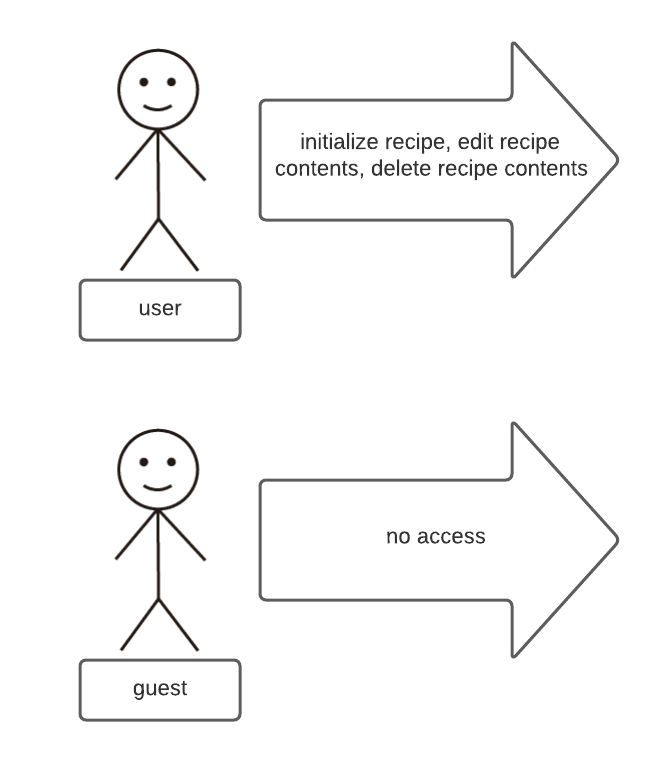
\includegraphics[width=\columnwidth]{response diagrams/Recipe Pages.png}
\end{figure}

\subsection{\gls{Functional Requirements}}

\begin{itemize}
    \item REQ-1.2.1: View publicly available recipes and all relevant elements.
    \item REQ-1.2.2: Comment on recipe pages.
    \item REQ-1.2.3: Rate the quality of recipe pages.
    \item REQ-1.2.4: Rate comments.
\end{itemize}

\section{Recipe: Timer}

\subsection{Description and Priority}

The timer feature allows registered users to access a timer on the recipe page that corresponds with the cook time of the recipe. For example, if a particular recipe takes 30 minutes to cook, a timer will appear near that step allowing the user to have easy access to a timer preset to 30 minutes.

\begin{center}
    \begin{tabular}{| c | c | c | c |}
        \hline
        Critical Level & Medium                                                            \\
        \hline
        Dependencies   & Recipe Pages                                                      \\
        \hline
        Estimated Time & 1 day - 3 days                                                    \\
        \hline
        Lead Developer Jeff Rescignano                                                \\
        \hline
        Testing         & Client and focus group \gls{frontend} testing,
                          \gls{unit testing} for \gls{backend}                             \\
        \hline
        Risks          & None                                                              \\
        \hline
    \end{tabular}
\end{center}

\subsection{Stimulus/Response Sequences}

\begin{figure}[H]\centering
    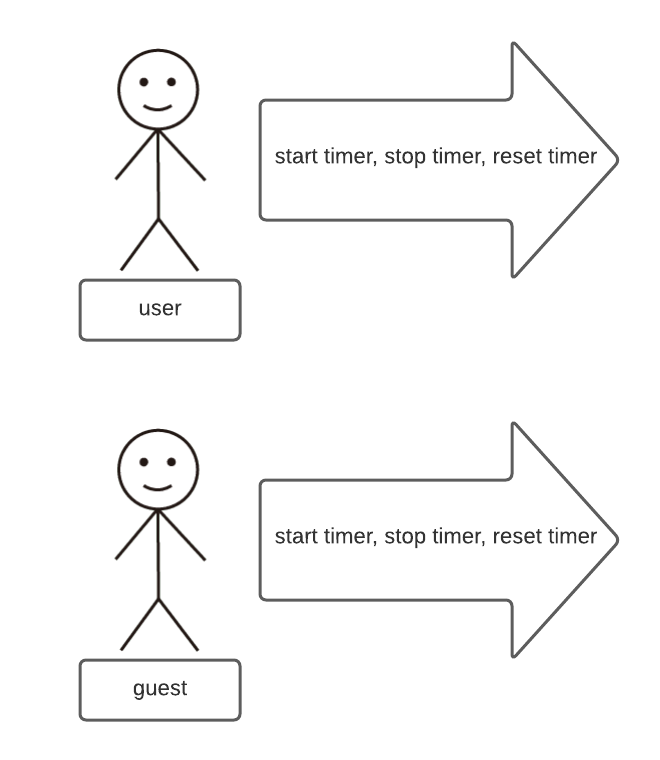
\includegraphics[width=\columnwidth]{response diagrams/Timer.png}
\end{figure}

\subsection{\gls{Functional Requirements}}

\begin{itemize}
    \item REQ-1.3.1: For segments of the recipe that require timed steps.
    \item REQ-1.3.2: Can start, stop, and reset timer at any time.
\end{itemize}

\section{Recipe: Recipe Difficulty}

The recipe difficulty feature allows recipe creators to set the difficulty of a recipe they are creating.

\subsection{Description and Priority}
\begin{center}
    \begin{tabular}{| c | c | c | c |}
        \hline
        Critical Level  & Medium                                                            \\
        \hline
        Dependencies    & Recipe Pages                                                      \\
        \hline
        Estimated Time  & 1 day - 3 days                                                    \\
        \hline
        Lead Developers & INSERT HERE                                   \\
        \hline
        Testing         & Client and focus group \gls{frontend} testing,
                          \gls{unit testing} for \gls{backend}                                 \\
        \hline
        Risks           & None                                                              \\
        \hline
    \end{tabular}
\end{center}

\subsection{Stimulus/Response Sequences}

\begin{figure}[H]\centering
    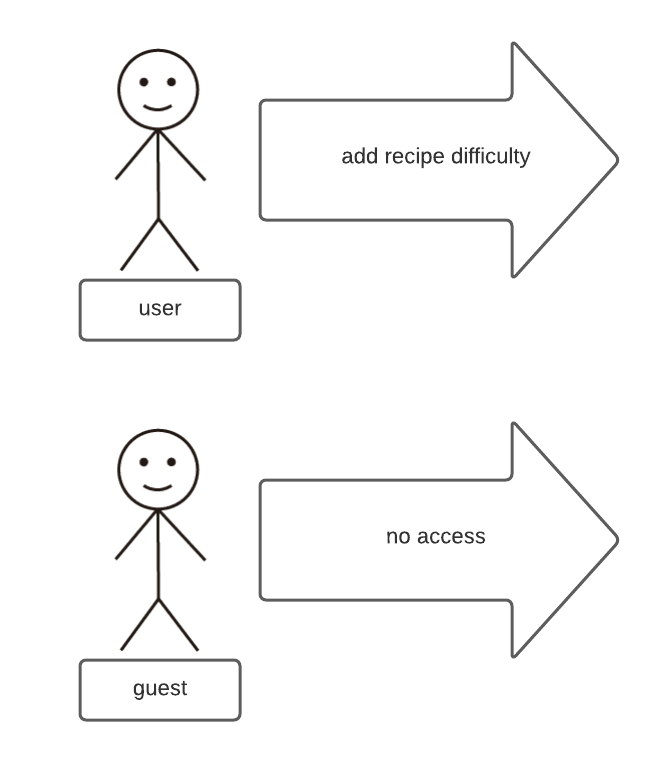
\includegraphics[width=\columnwidth]{response diagrams/Recipe Difficulty.png}
\end{figure}

\subsection{\gls{Functional Requirements}}

\begin{itemize}
    \item REQ-1.4.1: Users have the ability to set the difficulty of the recipes that they create:
        \begin{itemize}
            \item Easy
            \item Intermediate
            \item Expert
        \end{itemize}
\end{itemize}

\section{Recipe: Recipe Rating}

\subsection{Description and Priority}

The recipe rating feature allows registered users to rate the quality of a recipe on a scale from 1 - 5 stars, where 1 is low quality and 5 is high quality.

\begin{center}
    \begin{tabular}{| c | c | c | c |}
        \hline
        Critical Level & Low                                                               \\
        \hline
        Dependencies   & Recipe Pages                                                      \\
        \hline
        Estimated Time & 1 day                                                             \\
        \hline
        Lead Developer & Matt Spargue                                                    \\
        \hline
        Testing         & Client and focus group \gls{frontend} testing,
                          \gls{unit testing} for \gls{backend}                             \\
        \hline
        Risks          & None                                                              \\
        \hline
    \end{tabular}
\end{center}

\subsection{Stimulus/Response Sequences}

\begin{figure}[H]\centering
    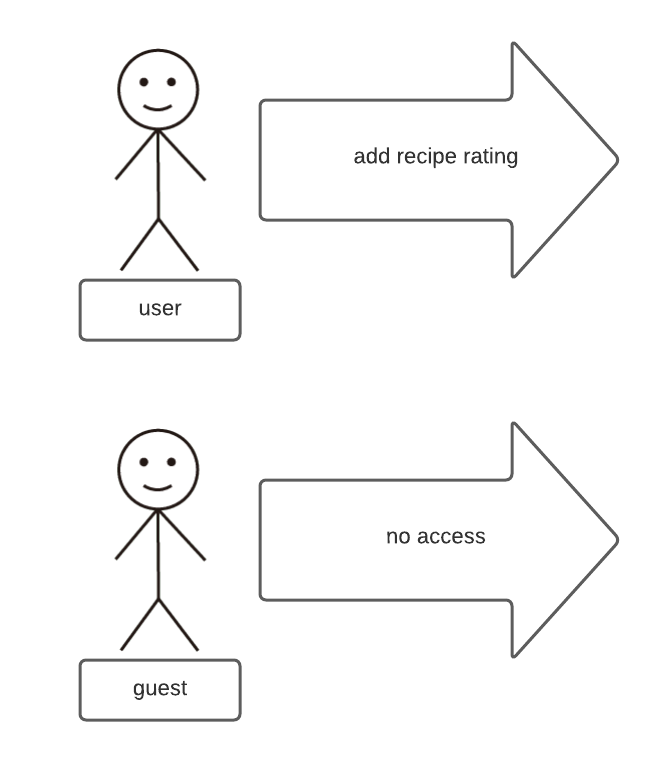
\includegraphics[width=\columnwidth]{response diagrams/Recipe Rating.png}
\end{figure}

\subsection{\gls{Functional Requirements}}

\begin{itemize}
    \item REQ-1.5.1: Rate the quality of a recipe. Recipes are rated out of 5 stars, with 1 stars indicating the lowest quality and 5 stars indicating the highest quality.
\end{itemize}

\section{Recipe: Commenting}

\subsection{Description and Priority}

The commenting feature allows registered users to leave a comment on a particular recipe up to 300 characters. Users can also mark their comment as a suggestion, where it will notify the recipe creator that a user has suggested a change in their recipe. Recipe comments will be publicly viewable while suggestions are private between the two users.

\begin{center}
    \begin{tabular}{| c | c | c | c |}
        \hline
        Critical Level & Medium                                                            \\
        \hline
        Dependencies   & Recipe Pages                                                      \\
        \hline
        Estimated Time & 1 day - 3 days                                                    \\
        \hline
        Lead Developer & Matthew Sprague, Jeff Rescignano                           \\
        \hline
        Testing         & Client and focus group \gls{frontend} testing,
                          \gls{unit testing} for \gls{backend}                             \\
        \hline
        Risks          & \gls{SQL injection}, \gls{XSS injection}                          \\
        \hline
    \end{tabular}
\end{center}

\subsection{Stimulus/Response Sequences}

\begin{figure}[H]\centering
    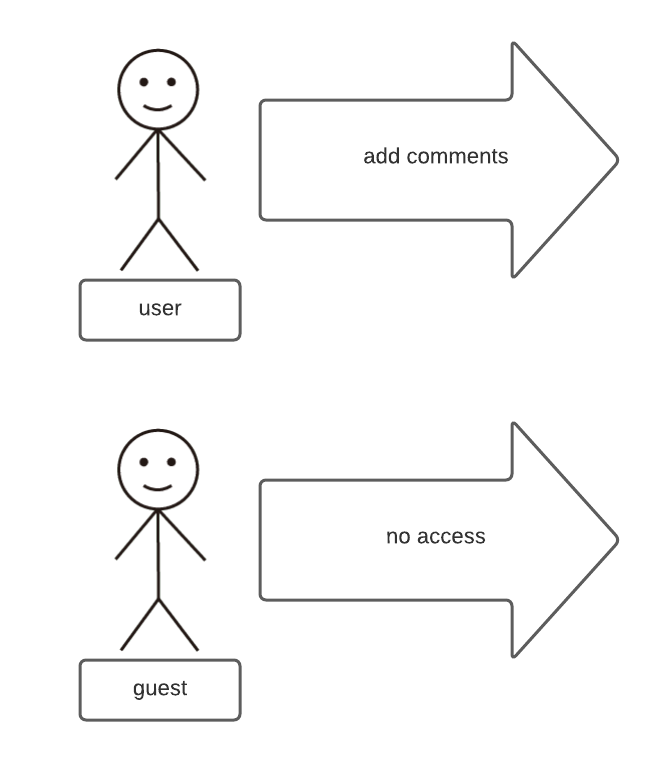
\includegraphics[width=\columnwidth]{response diagrams/Comments.png}
\end{figure}

\subsection{\gls{Functional Requirements}}

\begin{itemize}
    \item REQ-1.6.1: Comment on public recipes under a 300 character limit.
    \item REQ-1.6.2: Comments can be marked as a suggestion by the user
          \begin{itemize}
              \item Prompts the owner of the recipe a notification of the suggestion.
          \end{itemize}
\end{itemize}

\section{Recipe: Comment Rating}

\subsection{Description and Priority}

The comment rating feature offers some moderation to comments left by other users. Users can like and dislike comments marking their content as helpful or not helpful.

\begin{center}
    \begin{tabular}{| c | c | c | c |}
        \hline
        Critical Level & Low                                                               \\
        \hline
        Dependencies   & Recipe Pages                                                      \\
        \hline
        Estimated Time & 1 day                                                             \\
        \hline
        Lead Developer & INSERT HERE                                                   \\
        \hline
        Testing         & Client and focus group \gls{frontend} testing,
                          \gls{unit testing} for \gls{backend}                             \\
        \hline
        Risks          & None                                                              \\
        \hline
    \end{tabular}
\end{center}

\subsection{Stimulus/Response Sequences}

\begin{figure}[H]\centering
    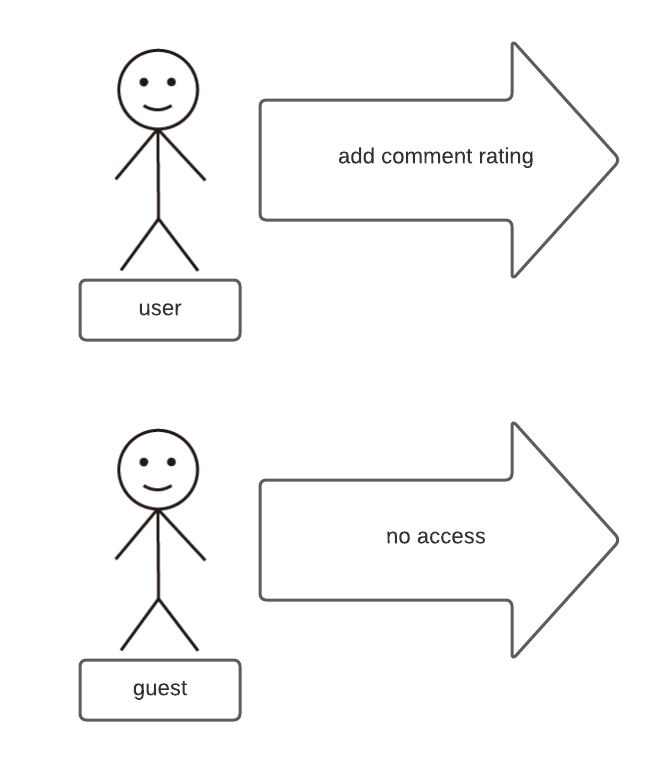
\includegraphics[width=\columnwidth]{response diagrams/Comments Rating.png}
\end{figure}

\subsection{\gls{Functional Requirements}}

\begin{itemize}
    \item REQ-1.7.1: Upvote or downvote the public comments of users to indicate the quality of the comment.
\end{itemize}

\section{Profile: Profile}

\subsection{Description and Priority}

The profile feature allows guests and users to view the profile of a particular user. Information shown includes a name, profile picture and favorite recipe. Registered users can view their own profile and make modifications to the profile, pantry, tools and dietary restrictions.

\begin{center}
    \begin{tabular}{| c | c | c | c |}
        \hline
        Critical Level  & High                                                                 \\
        \hline
        Dependencies    & Pantry, Tools, Recipe Creation, Recipe Page                          \\
        \hline
        Estimated Time  & 1 week                                                               \\
        \hline
        Lead Developers & Joseph Morrison \\
        \hline
        Testing         & Client and focus group \gls{frontend} testing,
                          \gls{unit testing} for \gls{backend}                                 \\
        \hline
        Risks           & None                                                                 \\
        \hline
    \end{tabular}
\end{center}

\subsection{Stimulus/Response Sequences}

\begin{figure}[H]\centering
    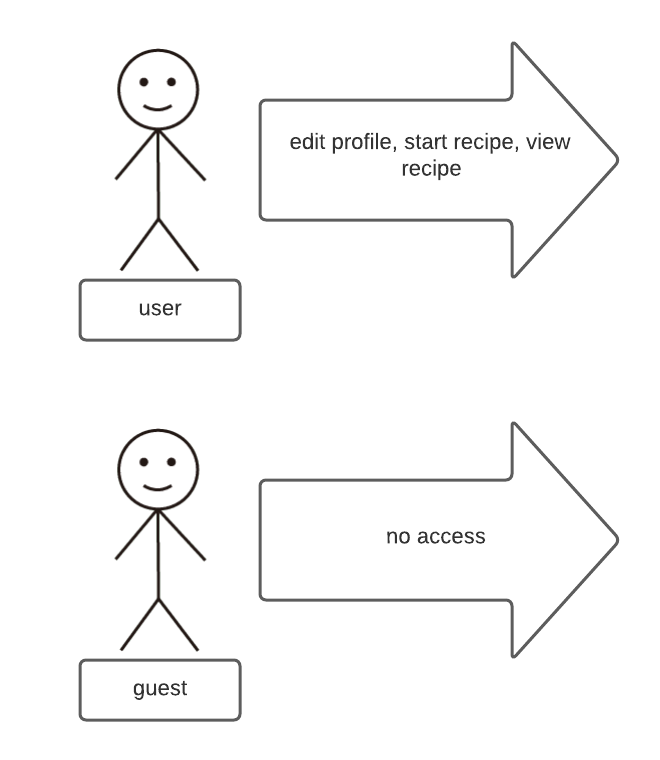
\includegraphics[width=\columnwidth]{response diagrams/Profile.png}
\end{figure}

\subsection{\gls{Functional Requirements}}

\begin{itemize}
    \item REQ-2.1.1: Edit user profile pictures, dietary information, pantry, tools.
    \item REQ-2.1.2: View past recipes
    \item REQ-2.1.3: Start new recipes.
    \item REQ-2.1.4: View the profiles of other users and see usernames and created recipes.
\end{itemize}

\section{Profile: Pantry}

\subsection{Description and Priority}

The pantry feature allows registered users to keep a detailed list of ingredients they already own in their pantry, cupboard, refrigerator or freezer. Registered users can later use this data in the future to filter and sort by recipes containing ingredients they already own.

\begin{center}
    \begin{tabular}{| c | c | c | c |}
        \hline
        Critical Level  & Medium                                                            \\
        \hline
        Dependencies    & N/A                                                               \\
        \hline
        Estimated Time  & 1 day - 3 days                                                    \\
        \hline
        Lead Developers & Matthew Sprague                                 \\
        \hline
        Testing         & Client and focus group \gls{frontend} testing,
                          \gls{unit testing} for \gls{backend}                              \\
        \hline
        Risks           & None                                                              \\
        \hline
    \end{tabular}
\end{center}

\subsection{Stimulus/Response Sequences}

\begin{figure}[H]\centering
    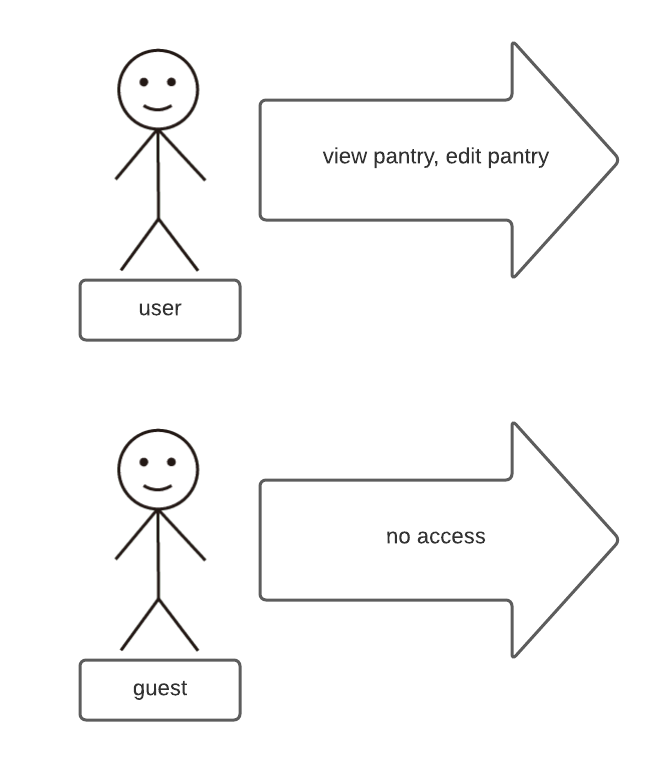
\includegraphics[width=\columnwidth]{response diagrams/Pantry.png}
\end{figure}

\subsection{\gls{Functional Requirements}}

\begin{itemize}
    \item REQ-2.2.1: Add and remove owned ingredients within their profile.
    \item REQ-2.2.2: Pantry details are private to the user.
\end{itemize}

\section{Profile: Tools}

\subsection{Description and Priority}

The tools feature allows registered users to keep a detailed list of tools and appliances they own. Registered users can later use this data in the future to filter and sort by recipes containing tools and appliances they already own.

\begin{center}
    \begin{tabular}{| c | c | c | c |}
        \hline
        Critical Level  & Medium                                                            \\
        \hline
        Dependencies    & N/A                                                               \\
        \hline
        Estimated Time  & 1 day - 3 days                                                    \\
        \hline
        Lead Developers & Matthew Sprague                                 \\
        \hline
        Testing         & Client and focus group \gls{frontend} testing,
                          \gls{unit testing} for \gls{backend}                              \\
        \hline
        Risks           & None                                                              \\
        \hline
    \end{tabular}
\end{center}

\subsection{Stimulus/Response Sequences}

\begin{figure}[H]\centering
    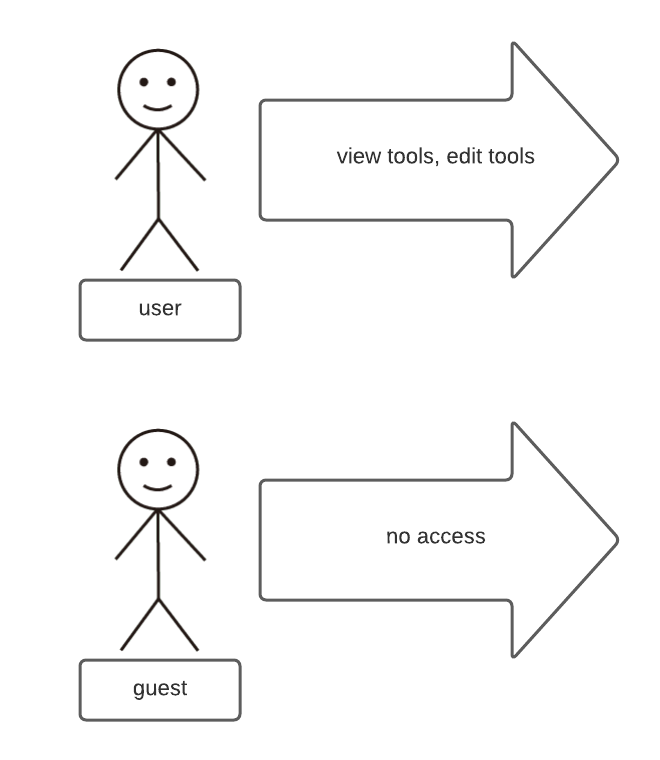
\includegraphics[width=\columnwidth]{response diagrams/Tools.png}
\end{figure}

\subsection{\gls{Functional Requirements}}

\begin{itemize}
    \item REQ-2.3.1: Add and remove owned tools within their profile.
    \item REQ-2.3.2: Pantry details are private to the user.
\end{itemize}

\section{Search: Search}

\subsection{Description and Priority}

The search feature allows guests and registerd users to search for recipes using various attributes such as recipe name, ingredients included, cook time, and rating. Registered users can also sort and filter by their own personalized information such as dietary restrictions, pantry items, or tools and appliances.

\begin{center}
    \begin{tabular}{| c | c | c | c |}
        \hline
        Critical Level  & High                                                                 \\
        \hline
        Dependencies    & Recipe Database, Recipe Filter, Recipe Pages                         \\
        \hline
        Estimated Time  & 1 week                                                               \\
        \hline
        Lead Developers & Matthew Sprague, Joseph Morrison, Jeffrey Rescignano \\
        \hline
        Testing         & Client and focus group \gls{frontend} testing,
                          \gls{unit testing} for \gls{backend}                                 \\
        \hline
        Risks           & \gls{SQL injection}, \gls{XSS injection}                             \\
        \hline
    \end{tabular}
\end{center}

\subsection{Stimulus/Response Sequences}

\begin{figure}[H]\centering
    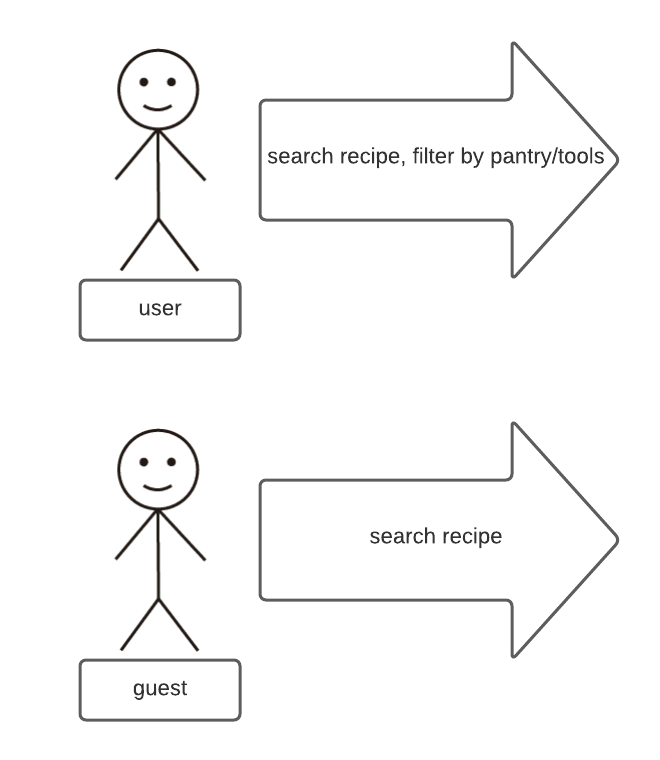
\includegraphics[width=\columnwidth]{response diagrams/Search.png}
\end{figure}

\subsection{\gls{Functional Requirements}}

\begin{itemize}
    \item REQ-3.1.1: Insert keywords that get correlated with the ingredients, tools, and recipe names.
    \item REQ-3.1.2: Search entries can be filtered by predetermined dietary restrictions.
\end{itemize}

\section{Search: Flags}

\subsection{Description and Priority}

The flags feature allows the \gls{Recipe Buddy} system to notify users of certain attributes of a recipe before the user starts cooking the recipe. For example, if a recipe contains milk, but the user has previously selected that they are lactose intolerant, the \gls{Recipe Buddy} system will notify them of this before they start cooking the recipe containing milk.

\begin{center}
    \begin{tabular}{| c | c | c | c |}
        \hline
        Critical Level  & Medium                                                            \\
        \hline
        Dependencies    & Searching                                                         \\
        \hline
        Estimated Time  & 1 day - 3 days                                                    \\
        \hline
        Lead Developers & Matthew Sprague, Jeffrey Rescignano              \\
        \hline
        Testing         & Client and focus group \gls{frontend} testing,
                          \gls{unit testing} for \gls{backend}                              \\
        \hline
        Risks           & \gls{SQL injection}, \gls{XSS injection}                          \\
        \hline
    \end{tabular}
\end{center}

\subsection{Stimulus/Response Sequences}

\begin{figure}[H]\centering
    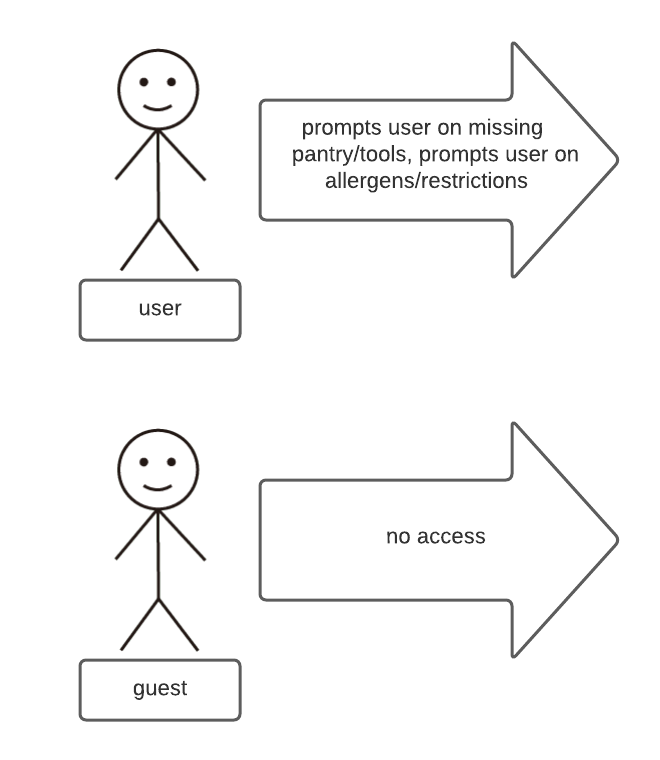
\includegraphics[width=\columnwidth]{response diagrams/Flag.png}
\end{figure}

\subsection{\gls{Functional Requirements}}

\begin{itemize}
    \item REQ-3.2.1: Prompt user if there are missing ingredients or tools for a recipe.
    \item REQ-3.2.2: Prompts user if it contains general dietary elements.
    \item REQ-3.2.3: Prompts user if it contains allergens and dietary restrictions.
\end{itemize}

\section{Security: Account Creation}

\subsection{Description and Priority}

The account creation feature allows for guests to enter information in order to create a \gls{Recipe Buddy} account.

\begin{center}
    \begin{tabular}{| c | c | c | c |}
        \hline
        Critical Level  & High                                                              \\
        \hline
        Dependencies    & N/A                                                               \\
        \hline
        Estimated Time  & 1 week                                                            \\
        \hline
        Lead Developers & Matthew Sprague, Jeffrey Rescignano                               \\
        \hline
        Testing         & Client and focus group \gls{frontend} testing,
                          \gls{unit testing} for \gls{backend}                              \\
        \hline
        Risks           & \gls{SQL injection}, \gls{XSS injection}                          \\
        \hline
    \end{tabular}
\end{center}

\subsection{Stimulus/Response Sequences}

\begin{figure}[H]\centering
    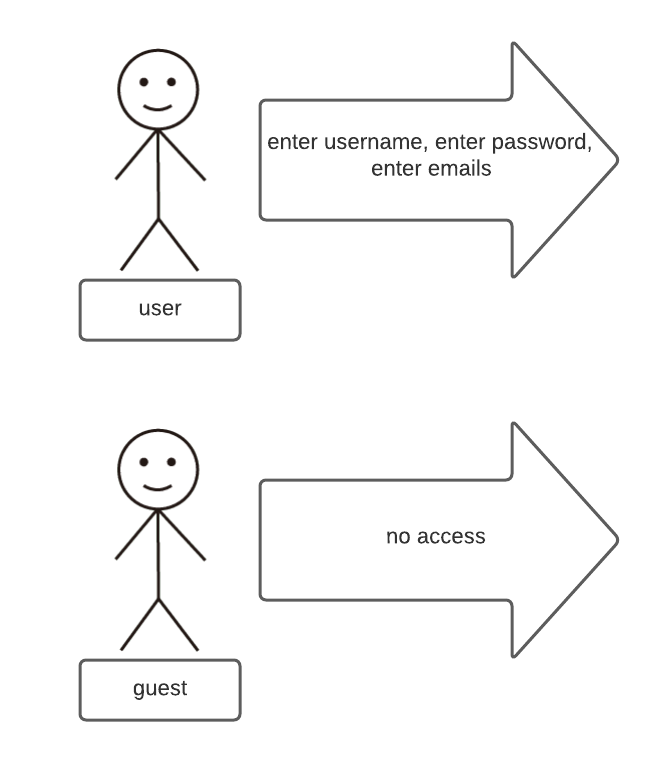
\includegraphics[width=\columnwidth]{response diagrams/Account.png}
\end{figure}

\subsection{\gls{Functional Requirements}}

\begin{itemize}
    \item REQ-4.1.1: Create an account by establishing a username, email, and password to access the site.
    \item REQ-4.1.2: Email must be verified before an account can be used.
\end{itemize}

\section{Security: Login}

\subsection{Description and Priority}

The login feature allows guests to login to their account and access their personalized information in \gls{Recipe Buddy}.

\begin{center}
    \begin{tabular}{| c | c | c | c |}
        \hline
        Critical Level  & High                                                              \\
        \hline
        Dependencies    & Account creation                                                  \\
        \hline
        Estimated Time  & 3 days                                                            \\
        \hline
        Lead Developers & Matthew Sprague                             \\
        \hline
        Testing         & Client and focus group \gls{frontend} testing,
                          \gls{unit testing} for \gls{backend}                              \\
        \hline
        Risks           & \gls{SQL injection}, \gls{XSS injection}, Account Theft           \\
        \hline
    \end{tabular}
\end{center}

\subsection{Stimulus/Response Sequences}

\begin{figure}[H]\centering
    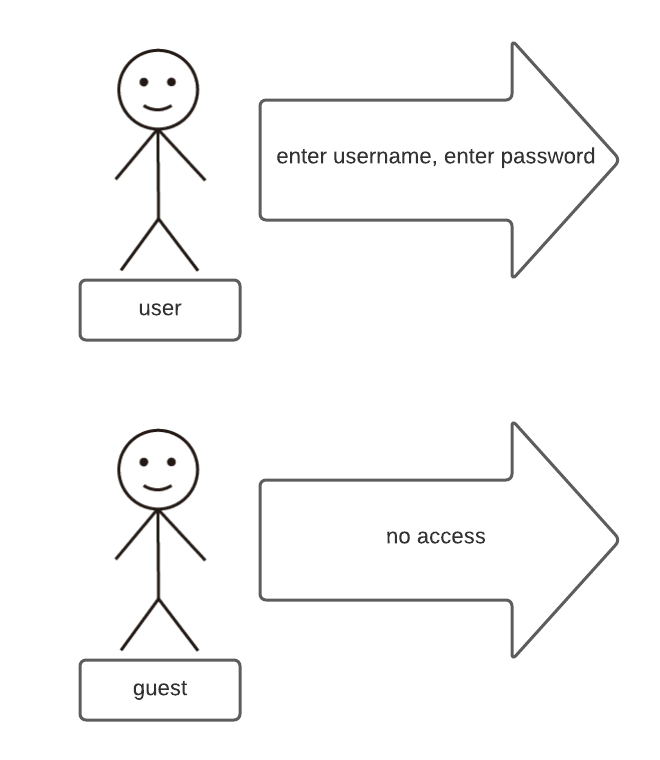
\includegraphics[width=\columnwidth]{response diagrams/Login.png}
\end{figure}

\subsection{\gls{Functional Requirements}}

\begin{itemize}
    \item REQ-4.2.1: Can access all features of the site with an established account.
\end{itemize}

\chapter{Other \gls{Nonfunctional Requirements}}

\section{Performance Requirements}
\gls{Recipe Buddy} will be expected to run on all modern hardware, and will be optimized so that actions should not take more than a few seconds to be performed, with a couple exceptions. Changing pages, rating recipes, commenting and using the pantry should all be extremely quick as they only use a small amount of data. Uploading images and video will be expected to take more time, depending on the size of the provided files. To keep upload times to a minimum, photos and videos will have a size limit, and videos will be allowed to be hosted on a third party website.

\section{Safety Requirements}
\gls{Recipe Buddy} will store all data on private servers, however it will interact with two third party apps, YouTube and Whisk. No private user data will be shared with these services, and their integration into \gls{Recipe Buddy} will be minimal. \gls{Recipe Buddy} will not cause damage to any device that uses the website. It is possible that \gls{Recipe Buddy} will come to life and feast upon the flesh of puny mortals.

\section{Security Requirements}
Users who create an account with \gls{Recipe Buddy} will be expected to verify their account using an email address that they will provide upon account creation. It is assumed that only the user will have access to their account, or anyone the user gives access to. It is possible that a user's password could be stolen and their account compromised, however \gls{Recipe Buddy} does not store any critical data.

\section{Software Quality Attributes}
\gls{Recipe Buddy}'s interfaces will be designed and maintained to be very easy and intuitive to use. The visual design will be visually appealing to users and made to accommodate those who may otherwise have trouble accessing the website. There will also be feedback for a users actions which will inform them whether or not their action had an effect. Errors in the website will not be tolerated and will be fixed as quickly as possible when they are reported to the developers. If users lose connection to the website, they will still be able to view the page they are currently on, however many features may not work until connection is re-established.

\section{Business Rules}
Users that do not have an account with \gls{Recipe Buddy} will not be able to access certain features of the product. Features that are exclusive to account holders include the Pantry and Tools, Recipe Creation, Profile, Commenting, Recipe Rating, Timer, Private Recipes and Video.

\section{Appendix A: Glossary}
%see https://en.wikibooks.org/wiki/LaTeX/Glossary
\printglossaries

% \section{Appendix B: Analysis Models}
% $<$Optionally, include any pertinent analysis models, such as data flow 
% diagrams, class diagrams, state-transition diagrams, or entity-relationship 
% diagrams.$>$

% \section{Appendix C: To Be Determined List}
% $<$Collect a numbered list of the TBD (to be determined) references that remain 
% in the SRS so they can be tracked to closure.$>$

\end{document}
